% Supplemental Appendix A algorithm source, not included in this section.
\resizebox{0.92\columnwidth}{!}{%
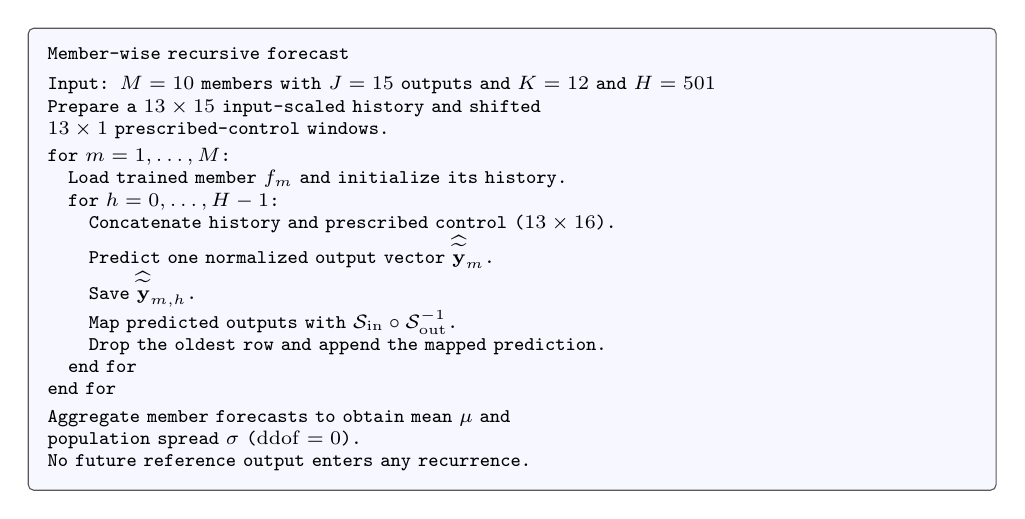
\begin{tikzpicture}[font=\ttfamily\scriptsize,draw=black!65]
 \node[draw,rounded corners=2pt,fill=blue!3,align=left,inner sep=7pt,text width=11.8cm] {%
   \textbf{Member-wise recursive forecast}\\[3pt]
   \textbf{Input:} $M=10$ members with $J=15$ outputs and $K=12$ and $H=501$\\
   Prepare a $13\times15$ input-scaled history and shifted\\
   $13\times1$ prescribed-control windows.\\[2pt]
   \textbf{for} $m=1,\ldots,M$:\\
   \quad Load trained member $f_m$ and initialize its history.\\
   \quad \textbf{for} $h=0,\ldots,H-1$:\\
   \qquad Concatenate history and prescribed control ($13\times16$).\\
   \qquad Predict one normalized output vector $\widehat{\widetilde{\mathbf y}}_m$.\\
   \qquad Save $\widehat{\widetilde{\mathbf y}}_{m,h}$.\\
   \qquad Map predicted outputs with $\mathcal S_{\mathrm{in}}\circ\mathcal S_{\mathrm{out}}^{-1}$.\\
   \qquad Drop the oldest row and append the mapped prediction.\\
   \quad \textbf{end for}\\
   \textbf{end for}\\[2pt]
   Aggregate member forecasts to obtain mean $\mu$ and\\
   population spread $\sigma$ ($\mathrm{ddof}=0$).\\
   No future reference output enters any recurrence.};
\end{tikzpicture}%
}
